\section{NVIDIA Collective Communications Library (NCLL)}

\begin{frame}{NCCL}
\begin{itemize}
\item NCCL is a communication library designed primarily for inter-GPU communications
\item It is not (currently) a stand alone parallel programming framework 
\item Generally, NCCL uses is very similar to MPI
\end{itemize}
\end{frame}

\begin{frame}{Why Do We NCCL}
	\begin{figure}
		\centering
		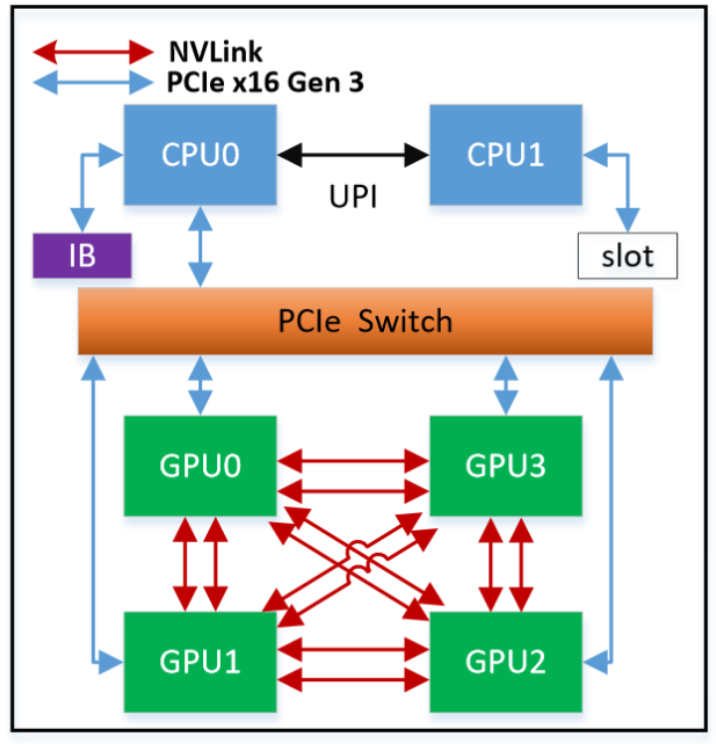
\includegraphics[width=0.45\linewidth]{figures/example_gpu_node_interconnect.png}
		\caption{An example of a possible multi-GPU node configuration}
	\end{figure}
\end{frame}

\begin{frame}[fragile]{NCCL Collective Operations}

\begin{minted}{c}
	// AllReduce
	ncclResult_t ncclAllReduce(const void* sendbuff, void* recvbuff, size_t count, ncclDataType_t datatype, ncclRedOp_t op, ncclComm_t comm, cudaStream_t stream)
	
	// Broadcast
	ncclResult_t ncclBroadcast(const void* sendbuff, void* recvbuff, size_t count, ncclDataType_t datatype, int root, ncclComm_t comm, cudaStream_t stream)
	
	// Reduce
	ncclResult_t ncclReduce(const void* sendbuff, void* recvbuff, size_t count, ncclDataType_t datatype, ncclRedOp_t op, int root, ncclComm_t comm, cudaStream_t stream)
	
	// AllGather
	ncclResult_t ncclAllGather(const void* sendbuff, void* recvbuff, size_t sendcount, ncclDataType_t datatype, ncclComm_t comm, cudaStream_t stream)
	
	// ReduceScatter
	ncclResult_t ncclReduceScatter(const void* sendbuff, void* recvbuff, size_t recvcount, ncclDataType_t datatype, ncclRedOp_t op, ncclComm_t comm, cudaStream_t stream)
\end{minted}
\end{frame}

\begin{frame}[fragile]{NCCL Point to Point Operations}
	
	Note, these are non-blocking.
	
	\begin{minted}{c}
		// Send
		ncclResult_t ncclSend(const void* sendbuff, size_t count, ncclDataType_t datatype, int peer, ncclComm_t comm, cudaStream_t stream)
		
		// Receive
		ncclResult_t ncclRecv(void* recvbuff, size_t count, ncclDataType_t datatype, int peer, ncclComm_t comm, cudaStream_t stream)
	\end{minted}
\end{frame}

\begin{frame}[fragile]{General Flow}
	
	\begin{minted}{c}
		// initialize MPI
		int myRank, nRanks, localRank = 0;
		MPI_Init(&argc, &argv);
		MPI_Comm_rank(MPI_COMM_WORLD, &myRank);
		MPI_Comm_size(MPI_COMM_WORLD, &nRanks);
		
		// initialize NCCL
		int nDev = 4;
		int devs[4] = { 0, 1, 2, 3 };
		ncclComm_t comms[4];
		ncclCommInitAll(comms, nDev, devs);
	\end{minted}
\end{frame}

\begin{frame}[fragile]{General Flow}
	
	\begin{minted}{c}
		// allocate and initializing device buffers
		float** sendbuff = (float**)malloc(nDev * sizeof(float*));
		float** recvbuff = (float**)malloc(nDev * sizeof(float*));
		cudaStream_t* s = (cudaStream_t*)malloc(sizeof(cudaStream_t)*nDev);
		
		
		for (int i = 0; i < nDev; ++i) {
			cudaSetDevice(i);
			cudaMalloc(sendbuff + i, size * sizeof(float));
			cudaMalloc(recvbuff + i, size * sizeof(float));
			cudaMemset(sendbuff[i], 1, size * sizeof(float));
			cudaMemset(recvbuff[i], 0, size * sizeof(float));
			cudaStreamCreate(s+i);
		}
	
	\end{minted}
\end{frame}

\begin{frame}[fragile]{General Flow}
	
	\begin{minted}{c}
		// Do some NCCL communication. Group API is required when using
		// multiple devices per thread
		ncclGroupStart();
		for (int i = 0; i < nDev; ++i)
		 	ncclAllReduce((const void*)sendbuff[i], (void*)recvbuff[i], size, ncclFloat, ncclSum,	comms[i], s[i]);
		ncclGroupEnd();
		
		
		// Make sure operations are synchronized by waiting for stream to finish
		for (int i = 0; i < nDev; ++i) {
			cudaSetDevice(i);
			cudaStreamSynchronize(s[i]);
		}
	\end{minted}
\end{frame}

\begin{frame}[fragile]{General Flow}
	
	\begin{minted}{c}
		// free device buffers
		for (int i = 0; i < nDev; ++i) {
			cudaSetDevice(i);
			cudaFree(sendbuff[i]);
			cudaFree(recvbuff[i]);
		}
		
		
		// finalizing NCCL
		for(int i = 0; i < nDev; ++i)
			ncclCommDestroy(comms[i]);
			
		// finalize MPI
		MPI_Finalize()
	\end{minted}
\end{frame}

\begin{frame}[fragile]{Example on M2}
	
	Run a simple benchmark on M2 from \url{https://github.com/NVIDIA/nccl-tests}
	
	\begin{minted}{sh}
		# get repository
		git clone git@github.com:NVIDIA/nccl-tests.git
		
		# change directory to the repository
		cd nccl-tests
		
		# load NVHPC module
		module load nvhpc-21.9
		
		# build with MPI enabled
		make MPI=1 CUDA_HOME=/hpc/applications/nvidia/hpc_sdk/2021_21.9/Linux_x86_64/21.9/cuda/11.4/
	\end{minted}
\end{frame}

\begin{frame}[fragile]{Run on 4 P100 nodes }
	\inputminted{sh}{examples/nccl/p100x4.sbatch}
\end{frame}

\begin{frame}[fragile]{Run on 4 P100 nodes }
	\inputminted{sh}{examples/nccl/p100x4.txt}
\end{frame}

\begin{frame}[fragile]{Run on 2 V100s on 2 nodes }
	\inputminted{sh}{examples/nccl/v100_2x2.sbatch}
\end{frame}

\begin{frame}[fragile]{Run on 2 V100s on 2 nodes}
	\inputminted{sh}{examples/nccl/v100_2x2.txt}
\end{frame}

\begin{frame}[fragile]{Run on 4 V100s on 1 node }
	\inputminted{sh}{examples/nccl/v100_4x1.sbatch}
\end{frame}

\begin{frame}[fragile]{Run on 4 V100s on 1 node}
	\inputminted{sh}{examples/nccl/v100_4x1.txt}
\end{frame}

